\section{Cross-Version Testing Study}
\label{sec:studylib}
In this section, we introduce our experimental study\footnote{Our data for this study and the following bug study are both available at \url{https://sites.google.com/site/incompemp2017/}.} on consecutive versions of Java libraries with cross-version testing. 

\subsection{Study Setup}
\subsubsection{Subject Libraries}
In our experimental study, we used 15 popular Java libraries as our subjects as shown in Column 1 of Table~\ref{table:basicInfo}. Specifically, we include in our subjects the two most widely used Java libraries: OpenJDK and the Android framework. Actually, since these two libraries have corresponding runtime platforms (i.e., JVM and Android OS), their BBIs are more likely to cause runtime errors, because the old version of client software may be executed in JVM or Android without recompile, and thus may result in runtime errors. Our subjects also include 7 libraries from Apache, and 6 other third-party libraries. All these libraries are from different domains and are the most popular software libraries in their domains according to a statistics~\cite{QSIC14}~\cite{techstat} of class imports among top 5,000 Java software projects in Github.

%To make our study results more representative, we performed a preliminary study on the usage of software libraries in 10,000 most popular (by the number of stars) Github Java projects. In each Java project, we checked the import statements in Java source files, and for each package prefix (first 3 terms in a package name, or the whole package name if it has less than 3 terms), we count it appears in the import statements of how many different projects. Then, we ranked the package prefixes, and did some manual adjustment (e.g., separating apache commons libraries by looking for first 4 terms, and merge multiple android and Java package prefixes). Finally, we acquired a list of most popular Java software libraries. 

%From the list, we choose the top 2 libraries: Java Runtime and Android Platform, as well as 25 other libraries that are open source, have sufficient test code, history long enough, and standard test code organization (i.e., Maven style organization of test code) to facilitate the automation of our study. Note that least popular library in our subject set ranked 41st in the list. 

\subsubsection{Selection of Version Pairs}
Software developers use different levels of versions to mark different granularity of milestones in software evolution. In our study, we first rule out the alpha and beta versions which are typically immature versions and are not widely used by client software developers. Then, we also need to differentiate major versions and minor versions. According to Semantic Versioning~\cite{SemVer}\cite{SCAM2014}, backward-incompatible API changes can be allowed in major versions (e.g., Java 6), but not minor versions (e.g., Java6u32). Also, major versions are typically developed in separate branches, while minor versions just corresponds to certain commits in the trunk or a branch. 

To acquire a full picture, in our study, we study backward incompatibilities both between two consecutive major versions and within a major version. If a major version has more than two minor versions, we choose the first minor version and the last minor version to form an inner-major-version version pair. For example, ElasticSearch has four minor versions (1.0.0 through 1.0.3) for major version 1.0, and three minor versions (1.1.0 through 1.1.2) for major version 1.1. So, in our study, we choose four versions (1.0.0, 1.0.3, 1.1.0, 1.1.2), and form 1 major version pairs (1.0.3 to 1.1.0) and two minor version pairs (1.0.0 to 1.0.3, 1.1.0 to 1.1.2). We combine minor versions within a major version because they typically contain very small amount of changes (e.g., fixing a bug), and may be inverted in the later updates if bringing in bugs or BBIs. So the combination will remove temporary BBIs (brought in and fixed with in a major version) which may not affect client developers much. We also ruled out the versions that raise compilation errors, or unit test failures / errors\footnote{For JDK and Android, we used the versions despite test failures and errors because some test cases require hardware support that we do not have. For JDK and Android versions, we ignore the test cases that fail on their own version.}. Finally, we use only versions up to Jan. 2015, so that their status  (e.g., documentation content) is relatively stable. Details of our selected versions as presented in Column 2-4 of Table~\ref{table:basicInfo} (Column 5-6 present the release time of the first and last version of the subject used in our study).

%, and the full list of version pairs used in our study are at our project website\footnote{\url{http://xywang.100871.net/empIncomp.html}}.
\begin{table}
	\center 
	\caption{\label{table:basicInfo} Basic Information of Studied Subjects and Versions}
	\begin{tabular}{|l|r|r|r|r|r|}
		\hline 
	      	Subject & St. V.& End V. & \# V.  & St. Time & End Time \\
    		\hline 
			OpenJDK & 7b157 & 8b13 & 2 &  2011-7 & 2014-3 \\
			Android & 4.3.1 & 5.0.1 & 2 &  2013-10 & 2014-12\\
			log4j & 2.0.0 & 2.1 &2 & 2014-7& 2014-10\\
			maven & 3.0.0 & 3.2.5 & 4& 2010-10& 2014-12\\
			bukkit &  1.2.3& 1.7.2 & 6& 2011-12 & 2013-12\\
			beanutils & 1.9.0 & 1.9.2 & 1 &  2008-9 & 2013-12\\
			codec & 1.6 & 1.7 & 1 &  2011-11 & 2012-9\\
			fileupload & 1.2.0 & 1.3.1 & 3 & 2007-2 & 2014-2\\
			commons-io & 2.0 & 2.4  & 4 & 2007-7& 2012-4\\
			ela. Search & 1.0.3 & 1.3.9 & 7& 2014-4& 2015-2\\
			http-core & 4.0.1 & 4.3.3 & 6& 2009-2 & 2014-2\\
			jodatime & 2.0  & 2.7 & 7 & 2011-5& 2015-1\\
			jsoup & 1.1.1 &1.7.3  & 10& 2010-6& 2013-11\\
			neo4j & 1.8.3 & 2.0.3 & 5&  2012-11& 2015-2\\
			snakeyaml & 1.3 & 1.11 & 8 &  2009-7 &2012-9\\
			\hline
	\end{tabular}
	\vspace{1cm}
\end{table}
%			antlr   & 3.0 & 3.5.2 & 7& 2007-5 & 2014-3\\ %
%			collections & 3.2.1 & 4.0 & 1& 2008-4 & 2013-11\\
%			cm-lang & 3.0.0 & 3.3.2 & 4&  2011-7 &2014-4\\
%			groovy & 1.0  & 1.8.8 & 9 & 2007-1 &2012-9\\
%			gson & 1.0 & 2.3 & 13 & 2008-5& 2014-8\\
%			guice & 1.0  & 3.0 & 2& 2007-3& 2011-3\\
%			hadoop & 2.0.0 &2.5  & 5& 2012-5 &2014-8\\
%			hibernate & 3.2 & 3.6.10 & 4& 2006-10& 2012-2\\
%			jfreechart & 1.0.14 & 1.0.19 & 5 & 2011-11& 2014-7\\
%			quartz & 1.7.0 & 2.2 & 8&  2010-2& 2013-9\\
%			slf4j & 1.1.0 & 1.7.10 & 11&  2006-12& 2015-1\\
%						cli & 1.1 & 1.2 & 1 & 2007-7 & 2009-3\\


%also tried to build and to run unit testing (using the version's own test code) on the versions, and
%Typically, ,minor versions corresponds to , and consecutive pairs (e.g., Java6u32 and Java6u40) of minor versions are not maintained simultaneously. 


%According to Semantic Versioning~\cite{semver}, \textit{Major Versions} as we consider Regarding mature versions, we observe that they mainly fall into two levels. The first level of versions involve major changes in software features and usages, and we refer to them as . Typically, , and consecutive pairs (e.g., Java 6 and Java 7) of major versions are maintained simultaneously by software developers . By contrast,  the second level of versions are mainly for bug fixes and minor changes inside a major version, and we refer to them as \textit{Minor Versions}. 



%Since the code difference between different levels of version pairs varies, the selection of version pairs may have a large impact to our study results. 




\subsubsection{Detection of BBIs}
\label{subsec:incompDetect}
%To detect signature incompatibilities, we simply compare the class / interface / method / field signatures, as well as inheritance hierarchies between a pair of versions, and calculate the difference. Note that, for simplicity and to avoid repetition, when counting member incompatibilities, we do not add the members that are removed due to class or hierarchy incompatibilities (i.e., removing a class results in removal of all its members, and removing an ancestor of a class results in removal of all the members inherited from the ancestor). Also, for a changed or removed member in a class, we count it for one member incompatibility in the class where the member is actually changed or removed, no matter how many sub-classes of the class are affected. 

Not all test cases in the old version compile with the source code of the new version (typically because they suffer from signature incompatibilities). Therefore, to detect behavioral incompatibilities, for each version pair, we automatically recompiled the test code of previous version with the source code of the new version, and iteratively remove the test cases that do not compile with the new version of source code, until all test cases can be compiled successfully. Finally, we executed all the remaining test cases and collected test failures and errors. Specifically, test compilation errors appear in 37 versions from 12 subjects (except for BeanUtils, FileUpload, and Codec), and in total 2,590 of 57,208 test cases (4.5\%) are removed due to compilations errors. 

Since one BBI may causes multiple test failures and errors, we further manually inspected these test failures and errors and grouped them into BBIs. For each test error/failure, we extracted the error messages, the version diff of the failed test code, and the version diff of the test class and the source class being tested. Then, we categorize multiple test errors/failures as one BBI if the test errors/failures are caused by the same API method and result in the same error message, exception, or wrong value of the same output/side effect. Note that, among 296 backward incompatibilities, library developers have revised test cases (e.g., changing test oracles or ways of invocation) for 267 incompatibilities, and deleted test cases for the other 11. For the rest 18 incompatibilities, change was made in other places of the test suite such as revising the setting up code or upgrading referred libraries. We found that revised test cases can help a lot in understanding the behaviors of BBIs. This categorization was done by first 2 authors separately, with the third author as a judge for conflicts. %Subjectivity is unavoidable in such an exploratory process, so we provide all test failures/errors and detailed categorization information on the project website, which supports replicate studies.

 
%\textbf{Clustering of Backward Incompatibility Groups.}
%To cluster test failures and errors in to incompatibility groups, we leverage the observation th at, if two test methods do not refer to the same set of methods in the source code of the software library, their failure must not be caused by the same backward incompatibility. It should be noted that, it is still possible that the behaviors of two methods in the software library change due to a same root cause. However, they are typically considered as two backward incompatibilities of the software library because two different APIs are affected. Therefore, in our algorithm, we first clustered all test cases in one test class to a cluster. The reason is that, they may fail due to a same error in the setup method of the test class. After that, for each pair of test classes, if they invoke a same method in the source code of the library, we deem them as interfered. Then, we clustered the test cases based on the closure of the interference relationship. For OpenJDK, there are two packages that are very commonly used: \CodeIn{java.lang} and \CodeIn{java.util}, so we ruled out methods in these packages when calculating interference, and manually inspected test failures / errors in test cases of these two packages. Note that the way we clustered backward incompatibilities is also conservative, which is consistent with the detection process. Therefore, we can guarantee that all of the identified incompatibility groups are truly incompatibility groups, and the number we report in this paper is an under-estimation of the number of behavioral backward incompatibilities. 


%simply check whether two test cases (failed or with error) 

\subsection{BBIs in Popular Libraries}
\label{subsubsec:prevIncomp}

To answer \textbf{RQ1}, we present the detected test failures / errors from software-library consecutive version pairs in Table~\ref{table:incompatibilities}. The first column of the table presents the subject name. Columns 2-3 present the total number of test failures detected in all version pairs of a specific subject (abbreviated as $T.$), and the number of versions where test failures are detected (denoted as $I$) divided by all version pairs of the subject (denoted as $A$). Columns 4-5 and 6-7 present similar data for test errors and BBIs (after grouping). Note that a test failure is raised when an assertion in the test case fails, while a test error is raised when the test case throws an unhandled exception or fails to complete. We also carefully checked the corresponding release notes, API documents, and migration guides (for Android) of the corresponding version pairs, and present the results in Column 8 of Table~\ref{table:incompatibilities}.


\begin{table}
	\center 
	\caption{\label{table:incompatibilities} BBIs in Software-Library Version Pairs}
		
		
	\begin{tabular}{|p{2.2cm}|R{1cm}|R{1.2cm}|R{1.15cm}|R{1cm}|R{1.1cm}|R{1cm}|R{1cm}|R{1.1cm}|R{1cm}|}
		\hline 
		Subject & \multicolumn{2}{c|}{Failure} & \multicolumn{2}{c|}{Error} & \multicolumn{3}{c|}{B-Incomp.} \\ 		
		\cline{2-8}
		        & T. & I/A  & T. & I/A  & T. & I/A & Doc. \\
        \hline
		OpenJDK & 203  & 2/2 & 15   & 2/2 & 35   & 2/2 & 13\\
		Android & 112  & 2/2 &  11  & 2/2 & 56  & 2/2 & 20\\ % 44 3 7 // 68 8 34
		log4j  &  21  & 2/2  & 0  & 0/2 & 4 & 2/2 &1\\			
		maven  & 14  & 3/4 & 226  & 4/4 & 19 & 4/4 &3\\		
		bukkit    & 15  & 2/6& 31  & 3/6 & 7  &4/6 &0\\		
		beanutils &  0 &  0/1 & 0  & 0/1 & 0  & 0/1 &0\\
		codec    & 4  &  1/1  & 6  & 1/1 & 6 & 1/1 &3\\
		fileupload & 0  & 0/3 & 12  & 2/3 & 2   & 2/3 & 0\\
		commons-io   &  4  & 1/4 & 2  & 1/4 & 3  & 2/4 & 0\\
		ela. Search  & 36   & 4/7 & 98  & 3/7 & 24  & 4/7 & 5\\
		http-core & 60  & 5/6 & 15  & 4/6 & 32  & 5/6 & 10\\		
		jodatime & 15   & 5/7 & 6  & 2/7 & 17  & 5/7 & 7\\
		jsoup  & 54  & 9/10 & 2   & 1/10  &  36  & 9/10 & 3\\
		neo4j   & 3   & 2/5 & 7  & 1/5 & 6 & 2/5 & 0\\
		snakeyaml & 108  & 8/8 & 14  & 4/8& 49& 8/8 & 17 \\
		\hline
		\NameEntry{2}{\textbf{Tot.}} & \NameEntry{2}{\textbf{649}} & \textbf{46/} & \NameEntry{2}{\textbf{445}}& \textbf{28/} &\NameEntry{2}{\textbf{296}} & \textbf{52/} & \NameEntry{2}{\textbf{82}}\\
		              &      & \textbf{68}  &      &  \textbf{68} &     & \textbf{68}&\\
		\hline
	\end{tabular}
\end{table}


From Table~\ref{table:incompatibilities}, we make our observation as follows. Considering that cross-version testing may generate an under approximation of the number of BBIs, the prevalence of BBIs may be much higher than what is shown in the table.


\medskip\vspace{+0.05cm}
\noindent\begin{tabular}{|p{16cm}|}
	\hline
	\textbf{Observation 1:} BBIs between version pairs are prevalent among Java software libraries. We detect 296 BBIs in 14 of 15 subjects (93.3\%), and 52 of 68 version pairs (76.5\%). Averagely each version pair suffers from 4.4 BBIs, and only 82 of the 296 BBIs are documented\\
	\hline
\end{tabular}
\medskip\vspace{+0.2cm}

%Second, on average, we detected 9.5 test failures, 6.5 test errors, and 4.4 BBIs for each version pair, showing that one version pair typically suffers from multiple BBIs. 




%\textbf{Documentation of BBIs.} 
%\begin{table}
	\center 
	\caption{\label{table:test-doc} Average Test Compilation Failures and Documented Incompatibilities cross Version Pairs}
	\begin{tabular}{|p{0.5cm}|r|r||r|r|}
		\hline 
		Sbj. & \multicolumn{2}{c||}{Comp. Status} & \multicolumn{2}{c|}{Documentation}  \\ 		
		\cline{2-5}
		        & \#No Comp. Error & \#All & \#Doc. BBI & \#All BBI \\
        \hline
		JDK & 5,940 & 6,212 & 14 & 35  \\
		and & 13,788 & 14,010 & 24 &  56 \\ % 44 3 7 // 68 8 34
		log  & 2,107 & 2,215 & 1  & 4   \\			
		mav  & 2,536 & 2,598 & 3 & 19 \\		
		buk    & 1,124 & 1,139  & 0& 7 \\		
		bea &  1,263 & 1,263 & 0 & 0  \\
		cod    & 408 & 408 &  1  & 6  \\
		fil & 25 & 25 & 0 & 2 \\
		cio   &  744  & 767 & 1 & 3 \\
		ela  & 14,347  & 16,220 & 5 & 24 \\
		htt & 5,726 & 6,322 & 3 & 32 \\		
		jod & 15  & 2.2 & 5 & 17 \\
		jso  & 54 & 5.4 & 5 & 36  \\
		neo   & 3 &  0.6  & 0 & 6 \\
		sna & 108 &13.5 & 8 & 49  \\
		\hline
		\textbf{Tot.} & \textbf{649} & \textbf{9.5} & \textbf{70} & \textbf{296}\\
		\hline
	\end{tabular}
	\vspace{1cm}
\end{table}



\textbf{Distribution of BBIs between / within major versions.} Beyond the overall status of backward incompatibilities between consecutive version pairs of software libraries, we further studied the difference between major and minor version pairs. The results are presented in Table~\ref{table:incompVersions}.
From Table~\ref{table:incompVersions}, we have the observation as follows. 

\medskip\vspace{+0.05cm}
\noindent\begin{tabular}{|p{16cm}|}
	\hline
	\textbf{Observation 2:} Major version pairs and minor version pairs suffered from 4.7 and 3.5 backward incompatibilities on average, respectively, and 76\% of both types of version pairs 
	are backward incompatible. Since BBIs are still prevalent within a major version, continuous minor version updates are still not safe, although they are slightly safer than major version upgrades. \\
	\hline
\end{tabular}
\medskip\vspace{+0.05cm}


\begin{table}
	\center 
	\caption{\label{table:incompVersions} Distribution of BBIs in Different Version Pairs}
		
		
	\begin{tabular}{|l|r|r|r|r|r|r|}
		\hline 
        Subject& 
        \multicolumn{2}{c|}{Total} & \multicolumn{2}{c|}{Average} & \multicolumn{2}{c|}{Incomp. V / All V}\\
        \cline{2-7}
                & Mj. & Mn. & Mj.  & Mn. & Mj. & Mn.        \\
        \hline
		JDK &  23 & 12 & 23 & 12   &  1/1 & 1/1  \\
		Android & 56 & N/A & 28 & N/A  & 2/2 &  N/A \\ % 44 3 7 // 68 8 34
		log4j  & 3  & 1 & 3  &  1   &  1/1 & 1/1  \\
		maven  &  10  & 9  & 5 & 4.5  & 2/2  & 2/2 \\
		bukkit & 3 & 4 & 0.8 & 2  & 3/4  & 1/2 \\
		beanutils & N/A & 0 & N/A & 0  & N/A &  0/1 \\
		codec & 6 &  N/A & 6 &  N/A &  1/1 & N/A \\
		fileupload & 0 & 2 & 0 & 1  & 0/1  & 2/2  \\
		commons-io  &  3 & N/A  & 0.8 & N/A &  2/4 & N/A  \\
		ela.Search  & 0  & 24 & 0 & 6  & 0/3 & 4/4 \\
		http-core &15  & 17 & 5 & 5.7 & 2/3 & 3/3 \\		
		jodatime  & 17 & N/A & 2.4 & N/A  &5/7  & N/A \\
		jsoup  & 31 & 5 & 4.4 & 1.2 &  7/7 & 3/4 \\
		neo4j  &  6 & 0 &  2  & 0  & 2/3 & 0/2  \\
		snakeyaml & 49 & N/A &4.9 & N/A & 10/10  & N/A \\
		\hline
		\textbf{Total} & \textbf{222} & \textbf{74} & \textbf{4.7} & \textbf{3.5} & \textbf{36/47}  & \textbf{16/21} \\
		\hline
	\end{tabular}
	\vspace{0.5cm}	
\end{table}



%To rule out signature-level incompatibilities, we delete the test cases that do not compile in our cross-version testing. Since major version pairs have more signature-level incompatibilities, less test cases are being used in cross-version testing. Therefore, the similar numbers in the table may not imply similar severity of backward incompatibility. However, the table does show that there are many backward incompatibilities between minor version pairs, which is not good news, because minor version pairs are typically supposed to be used for patching and minor changes, and are thus expected to be backward compatible. 

\subsection{Categorization of BBIs}
\label{subsec:cats}

To answer \textbf{RQ3}, we categorize BBIs according to their incompatible behaviors, invocation conditions, and the reasons why library developers brought them in. 

For the categorization of incompatibilities from 3 aspects (behaviors, invocation constraints, and reasons), it is exploratory so we do not have a criterion available beforehand. We predefined high-level categories (e.g. return value change as a high-level category of incompatible behaviors). Then, first 2 authors went through the incompatibilities separately and classify them to the categories. They also annotate each BBI with labels made up by themselves. Then, all authors discussed and merged labels with similar meanings, and removed too-narrow labels to get the final set of finer-grained categories. If we found a finer-grained category cannot be put into predefined high-level categories (e.g., Environment in Figure~\ref{figure:condition}), we made them separate high-level categories. Due to the complexity of BBIs, the categorization process is not easy, especially when the BBI involves multiple API methods. 

Consider Example~\ref{example:Method}, which is a test code sample from Jsoup 1.7.1. In the test case, an HTML document object is generated from HTML text, and then the document is printed out using \CodeIn{doc.body().html()} after setting char set to ascii and turn on escape mode. In Jsoup 1.7.3, the translation of some special characters for escape under ascii char set becomes different, so the printed HTML text will be changed. After inspection, we found that the change is made in method \CodeIn{html()}. Therefore, until \CodeIn{html()} is called, the memory status remains the same for both versions. In such a scenario, we determine that \CodeIn{html()} is the API method for the BBI, and the four API methods called before it are invocation constraint of the BBI. 

\begin{example}
	\begin{verbatim}
Document doc = 
    Jsoup.parse("<p title=p> & < > ...");
doc.outputSettings().charset("ascii");
doc.outputSettings().escapeMode();
assertEquals("...", doc.body().html());
	\end{verbatim}
	\caption{Identification of BBI-Related API Method} 
	\label{example:Method} 
\end{example}

\subsubsection{Incompatible Behaviors}

From the 296 BBIs, we identified the following major categories of incompatible behaviors. 

\textbf{Exceptions and Crashes} indicates that, in the new version of the software library, an API method throws exceptions in a different way. This category contains 4 sub-categories. \textit{New Exception} indicates that the API method throws an exception in the new version but not in the old version. \textit{Different Exception} indicates that the API method throws exceptions both versions, but the exceptions are different. \textit{No Exception} indicates that, the API method throws an exception in the old version, but not in the new version. \textit{Infinite Loop} indicates infinite loop in the new version. 

\textbf{Return Variable Change} indicates that, the return value of an API method changes in the new version under certain usage scenario and input. Specifically, we divide this category into four sub-categories. \textit{Value Change} indicates that a primitive value (e.g., integer, boolean, String) is changed. The BBI in Example~\ref{example:Method} belongs to this category. \textit{Field Change} indicates a field of the return object is changed. \textit{Type Change} indicates that the actual type of the return value is changed, although the signature itself remain unchanged. This typically happens when the return type in the API method signature has many subtypes (e.g., \CodeIn{java.lang.Object}). \textit{Structure Change} indicates that, no primitive values in the return object is changed, but the object is organized differently (i.e., values of reference-type fields or sub-fields of the return object are changed). 

\textbf{Other Effects} indicates that an API method causes a different side effect on other parts of the software itself or the operating system, such as value changes of other variables in \textit{Memory}, changes of the \textit{GUI}, and \textit{File System}. 

The distribution of 296 BBIs is presented in Figure~\ref{figure:behavior}. From the figure, we can see that the categories of \textit{Return Variable Change} and \textit{Exception and Crash} account for 162 and 105 BBIs, respectively, and they combined to account for more than 90\% of the BBIs. The two major subcategories for \textit{Return Variable Change} are changes of primitive return value or field value changes of object-type return values, which account for more than 90\% of the category. Such a distribution implies either most BBIs cause exceptions / simple return value changes, or such BBIs are more likely to be detected by regression testing. We will try to answer this question to some extent with our field bug study, but in either case, the following observation is true. 

\medskip\vspace{+0.05cm}
\noindent\begin{tabular}{|p{16cm}|}
	\hline
	\textbf{Observation 3:} Most BBIs detected by regression testing will cause either exceptions or value changes of the return variable or its fields, while side effects and environment effects are seldom detected.\\
	\hline
\end{tabular}
\medskip

%Another observation is that, incompatibilities detected in JDK and Android distribute more averagely amount all categories. The reason of the two observations may be, unhandled exceptions and value changes are more easily to be caught by unit testing. Since the test suites of JDK and Android are more comprehensive, they are able to detect incompatibilities in more various categories. 

%\begin{table}
 
	\caption{\label{table:Behave} Incompatible Behaviors}
	\begin{tabular}{|l|r|r|r|r|r|r|r|r|r|r|}
		\hline
		&  \multicolumn{4}{c|}{Exceptions}          &    \multicolumn{3}{c|}{Ret. Val. Change}  & \multicolumn{3}{c|}{Other Effects}\\
\cline{2-4} \cline{6-11}
Sbj. & UE & NE & DE & IL & VC & TC & SC & ME & UI & FS\\
\hline
JDK & 15 & 2 & 0 & 0 & 11 & 4 & 1 & 0 & 2 & 0\\
and & 9 & 6 & 2 & 3 & 19 & 1 & 3 & 3 & 6 & 4\\
log & 0 & 0 & 0 & 0 & 2 & 0 & 0 & 0 & 0 & 2\\
mav & 13 & 0 & 0 & 0 & 5 & 0 & 1 & 0 & 0 & 0\\
buk & 5 & 0 & 0 & 0 & 2 & 0 & 0 & 0 & 0 & 0\\
bea & 0 & 0 & 0 & 0 & 0 & 0 & 0 & 0 & 0 & 0\\
cod & 4 & 0 & 0 & 0 & 2 & 0 & 0 & 0 & 0 & 0\\
fil & 2 & 0 & 0 & 0 & 0 & 0 & 0 & 0 & 0 & 0\\
cio & 0 & 0 & 2 & 0 & 1 & 0 & 0 & 0 & 0 & 0\\
ela & 9 & 2 & 0 & 0 & 11 & 1 & 0 & 0 & 0 & 0\\
htt & 5 & 2 & 1 & 0 & 12 & 0 & 0 & 12 & 0 & 0\\
jod & 5 & 0 & 0 & 0 & 12 & 0 & 0 & 0 & 0 & 0\\
jso & 2 & 0 & 0 & 0 & 34 & 0 & 0 & 0 & 0 & 0\\
neo & 4 & 0 & 0 & 0 & 2 & 0 & 0 & 0 & 0 & 0\\
sna & 8 & 4 & 0 & 0 & 34 & 2 & 1 & 0 & 0 & 0\\
\hline
\textbf{Tot.} & \textbf{81} & \textbf{16} & \textbf{5} & \textbf{3} & \textbf{147} & \textbf{8} & \textbf{6} & \textbf{15} & \textbf{8} & \textbf{6}\\
\hline
	\end{tabular}	
	\vspace{1cm}
\end{table}
\begin{figure}
	\centering
	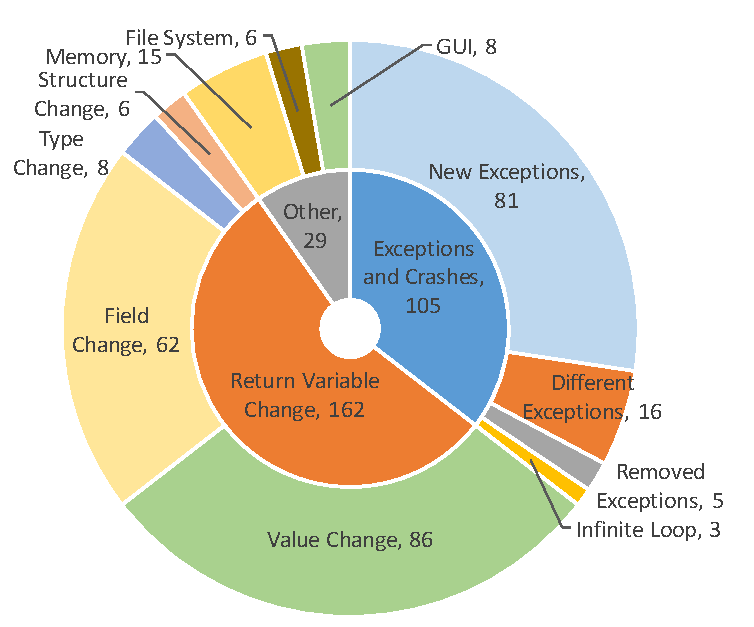
\includegraphics[width=0.4\textwidth]{backward/figs/Behavior.pdf}
	\caption{BBI Distribution on Incompatible Behaviors}
	\label{figure:behavior}
	\vspace{0.3cm}
\end{figure}

\subsubsection{Invocation Constraints}

We further investigated the conditions under which BBIs can be invoked, and identified the following five major types of such conditions. 

\textbf{Always} indicates that the BBI always happens as long as the corresponding API method is invoked.

%However, it should be noted that such incompatibilities may not be easily detected in the client software, because the relevant API method may not easily invoked, and the incompatible behavior (e.g., changed return value) may be overwritten by other code and thus cannot be observed under certain conditions. %Such incompatibilities can be easily detected by regression unit testing, so they are more likely to be intended behavioral changes.

\textbf{Error} indicates that the BBI happens only when an error happens. An example is the change of error message when a network error is invoked. 

\textbf{Environment} indicates that the BBI happens only under certain environments of the application (e.g., operating systems, language settings). 

\textbf{Multiple APIs} indicates that a number of other API methods must be invoked before the backward incompatible API method to invoke the BBI. Example~\ref{example:Method} belongs to this category. 

\textbf{Input} indicates that the BBI happens when a certain input value is fed into the corresponding API method. Specifically, we divide this category into five sub-categories. \textit{Trivial Value} indicates a null pointer or an empty string / list as the input. \textit{String Format} indicates that strings with specific structure as the input. \textit{Special Field} indicates that objects with specific values at a certain field as the input. \textit{Special Value} indicates that certain primitive values (not including strings) as the input. \textbf{Special Type} indicates the argument of the API method must be of a specific subtype of its parameter type.

The distribution of 296 backward incompatibilities in the above categories is presented in Figure~\ref{figure:condition}. We can observe that, the top 3 categories of invocation conditions are \textit{Always}, \textit{Specific Value}, and \textit{String Format}. The commonality among the 3 categories of BBIs is that they can be invoked with one API method invocation. By contrast, the BBIs requiring multiple API methods to invoke are not common in those detected by regression testing. 


%253 of 296 (85.5\%) detected BBIs alway happen whenever the API method is invoked, or happen under certain inputs. In the \textit{input} category, 129 BBIs are invoked by simple input values, while the rest 32 are fields of complicated inputs. 



%The dominance of category \textit{Always (\textbf{AL})} may be because they are easier to detect.

%Also, we observed that the distribution of categories in some projects are uneven. For example, JSoup, as the most popular HTML parser with 36 incompatibilities in total, contributes 30 of the 43 incompatibilities in the category of  \textit{String Format (\textbf{SF})}. Actually, while incompatibilities are distributed evenly in general libraries like JDK and Android. For library of narrower usage such as JSoup, Elastic Search and SnakeYaml (a data presentation library), more than 70\% of incompatibilities concentrate in \CodeIn{Jsoup.parse()}, \CodeIn{Client.prepareSearch()} and \CodeIn{Yaml.dump()}, the most widely used APIs in the libraries. 

%\begin{table}
	\center 
	\caption{\label{table:Cond} Invocation Conditions of Incompatibilities}
	\begin{tabular}{|l|r|r|r|r|r|r|r|r|r|}
		\hline
		&        &                &             &            &              & \multicolumn{4}{c|}{Input}\\
		\cline{7-10}
Subject & AL & ER & EV & ST & MA & TR & SF & FI & SV\\
\hline
JDK & 2 & 2 & 2 & 0 & 6 & 2 & 2 & 6 & 13\\
and & 18 & 4 & 2 & 1 & 4 & 11 & 3 & 4 & 9\\
log & 2 & 0 & 0 & 1 & 0 & 0 & 0 & 0 & 1\\
mav & 13 & 0 & 0 & 0 & 0 & 0 & 6 & 0 & 0\\
buk & 5 & 0 & 0 & 0 & 0 & 1 & 0 & 0 & 1\\
bea & 0 & 0 & 0 & 0 & 0 & 0 & 0 & 0 & 0\\
cod & 2 & 0 & 0 & 0 & 0 & 0 & 0 & 0 & 4\\
fil & 2 & 0 & 0 & 0 & 0 & 0 & 0 & 0 & 0\\
cio & 1 & 2 & 0 & 0 & 0 & 0 & 0 & 0 & 0\\
ela & 6 & 2 & 0 & 2 & 4 & 2 & 1 & 7 & 0\\
htt & 8 & 4 & 0 & 0 & 3 & 3 & 0 & 7 & 7\\
jod & 5 & 1 & 0 & 0 & 0 & 8 & 0 & 0 & 3\\
jso & 0 & 1 & 0 & 0 & 2 & 1 & 30 & 0 & 2\\
neo & 3 & 0 & 0 & 0 & 0 & 1 & 0 & 2 & 0\\
sna & 25 & 2 & 0 & 6 & 2 & 2 & 1 & 6 & 5\\
\hline
\textbf{Total} & \textbf{92} & \textbf{18} & \textbf{4} & \textbf{10} & \textbf{21} & \textbf{31} & \textbf{43} & \textbf{32} & \textbf{45}\\
\hline
	\end{tabular}
		\vspace{1cm}
\end{table}
\begin{figure}
	\centering
	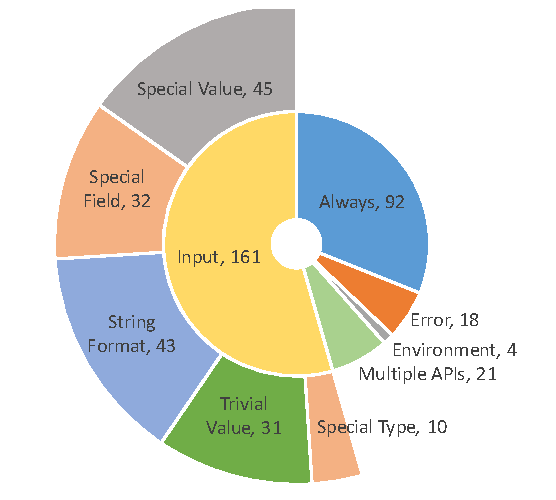
\includegraphics[width=0.4\textwidth]{backward/figs/Condition.pdf}
	
	\caption{BBI Distribution on Invoking Conditions}
	
	\label{figure:condition}
	\vspace{0.3cm}
\end{figure}


\subsubsection{Reasons for Bringing in BBIs}

Since the library developers revised the test cases to accommodate the changes, we can find out the reasons and the purposes of the behavior change from the revised test code. We identified the following 3 major categories of reasons, which contains 13 sub-categories. 

\textbf{Usage Change} indicates that the library developers expect to keep the normal behavior of the library, but also expect client developers to change their usage pattern. This category has 4 sub-categories, which are \textit{API Pattern Change} indicating changes on expected API sequences, \textit{Enforce Rules} indicating rejecting of some poor input, \textit{Enable Poor Inputs} indicating the support to some poor input, and \textit{Input Format} indicating the change on the format of string type inputs. 

\textbf{Better Output} indicates that the library developers expect to change the normal behavior of the API, while not expecting client developers to change their input. This category also has 5 sub-categories, which are \textit{More Reasonable Output/Effect} indicating behavior change of an API method under a normal input to make it more reasonable\footnote{For example, in log4j 2.0.2, the time stamp on the log is changed from when the log is initialized to when the time stamp line is printed. }, \textit{Change Default Setting} indicating changing of the default setting (often a constant such as the default screen size), \textit{Error Message} indicating change of reported errors, \textit{Explicit Report} indicating explicitly throwing exceptions for errors, and \textit{Output Format} indicating format change of string output. 

\textbf{Other} indicates reasons not in the above 2 categories, including \textit{Exposure of Internal Structure Change}, \textit{Signature Change exposed with Reflection}, and \textit{Upgrade Library}, in which the first two categories are regression faults.  

The distribution of 296 backward incompatibilities in the above categories is presented in Figure~\ref{figure:reason}. From the table, we can see the top 3 reasons for bringing incompatible behaviors are \textit{More Reasonable Output/Effect}, \textit{Output Format}, and \textit{Enforce Rules}. We also find that, \textit{Enable Poor Inputs}, the opposite of \textit{Enforce Rules}, is the 4th popular reasons. Such contradiction reflects hesitation of library developers on whether responsibilities (e.g., input validation checking) should be at the library side or client side. Also, we did observe library developers moving back-and-forth on some incompatibilities. For example, in SnakeYaml, whether the dump output should include class name of the data value is changed 3 times through versions 1.3 to 1.6. Furthermore, although \textit{More Reasonable Output/Effect} is the largest sub-category in \textit{Better Output}, 93 of 165 BBIs in the category are not semantic changes, but presentation changes (e.g., error message, explicit exceptions, output formats). The 17 BBIs on change of default setting also related to client developers' preference. To sum up, we have the following observation. 

\medskip\vspace{+0.05cm}
\noindent\begin{tabular}{|p{16cm}|}
	\hline
	\textbf{Observation 4:} Developers bring in a large portion of BBIs because they want to allow more or less inputs, or change the output presentation or option. This implies that the root cause of most BBIs is the different requirement of client developers, so the BBIs can be avoided if library developers understand requirement better (e.g., through surveys or code statistics on client projects), or have design for dual support.
	\\
	\hline
\end{tabular}
\medskip

%\begin{table}
\centering
	\caption{\label{table:reason} Reasons for Bringing in Incompatibilities}
	\begin{tabular}{|p{0.5cm}|R{0.5cm}|R{0.5cm}|R{0.5cm}|R{0.5cm}|R{0.5cm}|R{0.5cm}|R{0.5cm}|R{0.5cm}|R{0.5cm}|R{0.5cm}|R{0.5cm}|R{0.5cm}|R{0.5cm}|}
		\hline
		&  \multicolumn{5}{c|}{Usage Change}      &   \multicolumn{5}{c|}{Behavior Change}  & \multicolumn{3}{c|}{Other}\\
		\cline{2-14}
Sbj & AP & ER & EL & RE & IF & RB & CD & EM & DE & OF & IS & SR & UL\\
\hline
jdk & 6 & 13 & 3 & 1 & 0 & 7 & 2 & 0 & 1 & 1 & 1 & 0 & 0\\
and & 4 & 6 & 8 & 1 & 0 & 14 & 8 & 0 & 3 & 7 & 2 & 3 & 0\\
log & 2 & 1 & 0 & 0 & 0 & 1 & 0 & 0 & 0 & 0 & 0 & 0 & 0\\
mav & 0 & 0 & 1 & 1 & 0 & 2 & 0 & 1 & 0 & 0 & 1 & 1 & 12\\
buk & 0 & 1 & 0 & 0 & 0 & 0 & 0 & 0 & 0 & 2 & 0 & 4 & 0\\
bea & 0 & 0 & 0 & 0 & 0 & 0 & 0 & 0 & 0 & 0 & 0 & 0 & 0\\
cod & 0 & 4 & 0 & 0 & 0 & 2 & 0 & 0 & 0 & 0 & 0 & 0 & 0\\
fil & 0 & 0 & 0 & 0 & 1 & 0 & 0 & 0 & 0 & 0 & 0 & 0 & 1\\
cio & 0 & 0 & 0 & 0 & 0 & 1 & 0 & 0 & 2 & 0 & 0 & 0 & 0\\
ela & 1 & 2 & 3 & 5 & 0 & 3 & 1 & 4 & 0 & 2 & 1 & 2 & 0\\
htt & 2 & 4 & 5 & 3 & 1 & 10 & 2 & 0 & 1 & 4 & 0 & 0 & 0\\
jod & 0 & 3 & 1 & 6 & 1 & 0 & 1 & 0 & 1 & 3 & 1 & 0 & 0\\
jso & 0 & 2 & 8 & 0 & 3 & 13 & 0 & 0 & 0 & 10 & 0 & 0 & 0\\
neo & 0 & 3 & 1 & 0 & 0 & 1 & 1 & 0 & 0 & 0 & 0 & 0 & 0\\
sna & 2 & 2 & 3 & 2 & 0 & 1 & 2 & 16 & 1 & 15 & 3 & 2 & 0\\
\hline
\textbf{Tot.} & \textbf{17} & \textbf{41} & \textbf{33} & \textbf{19} & \textbf{6} & \textbf{55} & \textbf{17} & \textbf{21} & \textbf{9} & \textbf{44} & \textbf{9} & \textbf{12} & \textbf{13}\\
\hline
	\end{tabular}	
	\vspace{1cm}
\end{table}

\begin{figure}
	\centering
	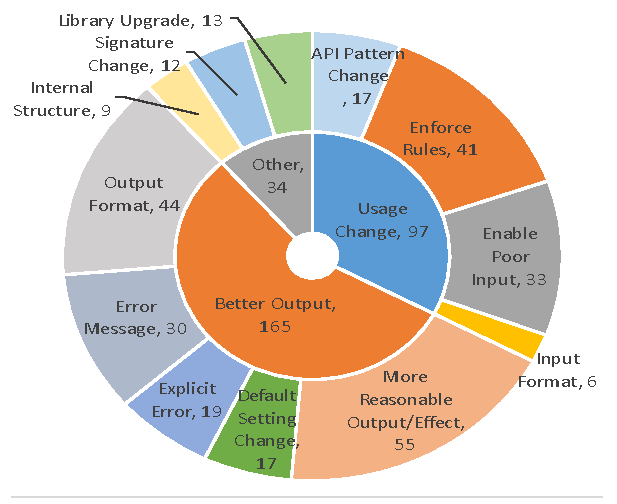
\includegraphics[width=0.4\textwidth]{backward/figs/Reason.pdf}
	
	\caption{BBI Distribution on Reasons}
	
	\label{figure:reason}
	\vspace{0.3cm}
\end{figure}
